\section{Présentation des problématiques}\label{sec:intro:problematique}
Contrairement aux approches actuelles, nous considérons comme acquis la capacité à dialoguer d'une manière ou d'une autre avec le système pour récolter les données. La figure~\ref{fig:intro:objectif:abstraction} représente la couche d'abstraction du système, permettant un accès unifié aux données. Le système est considéré comme un ensemble de sources de données qu'il est nécessaire de maîtriser. Dans cette section nous présentons les problématiques soulevés par l'observation de systèmes génériques.

\begin{figure}[ht]
\centering
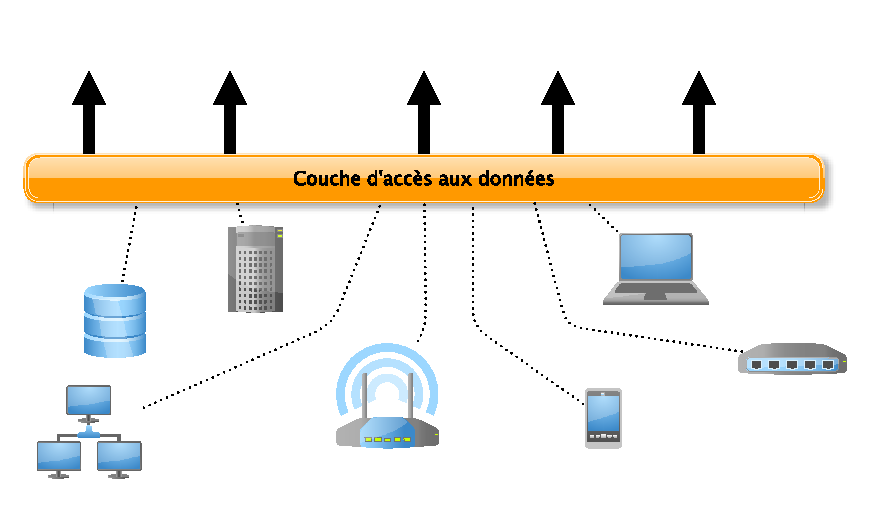
\includegraphics[width=0.7\textwidth]{intro-objectif}
\caption{Couche d'abstraction du système pour donner accès aux données}\label{fig:intro:objectif:abstraction}
\end{figure}

\subsection{Hétérogénéité des systèmes}
Plus l'informatique évolue, plus le nombre de dispositifs créés varie. Grâce à l'émergence de l'informatique ubiquitaire, les dispositifs se font de plus en plus nombreux et de natures complètement différentes. Ces caractéristiques rendent leur observation plus délicate car la surveillance des données d'un capteur est sensiblement différente à celle de l'utilisation d'un service d'hébergement web sur un serveur grande capacité.

Ainsi, il est nécessaire d'être capable de représenter toute sorte de système. Pour cela, il est nécessaire de définir un \textbf{schéma de données} reposant sur un \textbf{modèle de données}. Ce schéma détermine la sémantique accordé au système. Par exemple, en gestion de base de données, un modèle entité-relation détermine la représentation logique du système. Elle est par la suite traduite de façon physique en tables. En système d'information, la représentation d'un système passe souvent par un modèle objet. Cette capacité à représenter le système est critique pour manipuler clairement les concepts et leurs liens.

\subsection{Évolution des données du système}
Le système n'est pas statique dans le temps, c'est même souvent sa dynamique qui en fait sa richesse. Toutefois, cela introduit des problèmes majeurs d'un point de vue gestion des données. En effet, dans un système il existe deux grandes \textbf{catégories de données} : les données archivées et les données temps-réel. Les données archivés sont à évolution lente mais permet l'accès à des analyses de haut-niveau. Les données temps-réel sont des relevés instantanées et très volatiles indiquant l'état des entités du système (sous forme de flux de données).

Néanmoins, en l'état, chacune de ces catégories possède des modèles de données et des traitements propres. Or, ces données font toutes parties du même système. Nous pouvons remarquer qu'il existe des ponts naturels entre ces types. En effet, les approches classiques de surveillance par l'archive et l'analyse a posteriori montre qu'un flux nécessite d'être considéré comme un tout. De la même manière, une donnée stockée peut subir des modifications déclenchant la production d'événements, assimilables à des flux de données.

La création des processus de traitements de données est assimilable à une interrogation que pose l'utilisateur sur l'ensemble des données. Il existe différentes \textbf{modes d'interrogations} (ou requêtes). Celles-ci reflètent l'hétérogénéité de l'évolution des données.
\begin{itemize}
    \item \textbf{Interrogation instantanée} : C'est la manière usuelle d'interroger dans les applications de gestion de base de données. L'utilisateur pose une question sur un ensemble de données considérées figées, du moins le temps du calcul de la réponse. Le système fournit une réponse représentative d'un état à un instant donnée. Un exemple simple : \enquote{\it quel est l'ensemble actuel des équipements actifs de mon système}. La réponse à cette requête pourrait être \enquote{\it à cet instant, les équipements Box, PC1 et STB sont connectés et actifs}. La mention \enquote{\it à cet instant} est très importante, car si un nouvel équipement arrive dans le système, une nouvelle évaluation donnerait une réponse différente. Ainsi, cette interrogation correspond à la consultation ponctuelle de l'ensemble des données disponibles.
    \item \textbf{Interrogation continue} : C'est l'élément principal des systèmes événementiels, où les données sont considérés en constante évolution. L'utilisateur obtient ainsi une réponse qui évolue au cours du temps, sous forme de flux ou de mise à jour d'état. Un exemple pouvant être : \enquote{\it le flux de la charge processeur moyenne sur une minute du PC1}. La réponse forme un flux continu d'information qui, toutes les minutes, reporte une nouvelle valeur moyenne pour ce capteur. Ainsi, la formation de processus de collecte ou de formation d'alerte suivent ce type d'interrogation.
\end{itemize}

Il est important de noter que ces deux grands paradigmes d'interrogation peuvent se combiner. Par exemple, il est possible d'effectuer un appel à une interrogation instantanée à l'intérieur d'un processus continu. De façon similaire, l'appel régulier d'une interrogation instantanée forme une réponse continue. Il est nécessaire que le système d'observation soit capable de manipuler naturellement ces deux types d'interrogations pour manipuler correctement le dynamisme des données.

\subsection{Hétérogénéité des données et traitement}
La couche d'accès aux données permet d'exposer un ensemble de sources. Ces sources sont hétérogènes en terme de schéma et de nature (flux, archive).

Pour permettre une bonne compréhension du système et de ses interactions, il est nécessaire d'\textbf{intégrer} les différentes sources d'informations en une seule base d'information. En effet, chaque source de donnée peut-être considérée comme un fragment de cet ensemble. Ainsi, le système doit se doter de fonctionnalités d'agrégations de plusieurs sources.

L'\textbf{expression} des traitements possibles se fait à travers d'un \textbf{langage}. Son paradigme sous-jacent définit la manière et la facilité d'adaptation à un système en particulier. Ce langage peut être dans le cas le plus extrême : un langage de programmation impératif bas niveau (comme le C par exemple). Dans ce cas, l'approche est très algorithmique, permettant une meilleure gestion des performances, mais une utilisation plus difficile et technique par la suite. À l'autre extrême, le langage peut être issu de la programmation logique permettant des performances moins contrôlées, mais une gestion globale déclarative, permettant une grande flexibilité.

Le langage utilisé dans le système d'observation peut avoir un \textbf{pouvoir d'expression} limité. Il est important d'être capable d'énumérer ce qui est possible, ou non, d'exprimer en terme de processus. Les classes de logiques ou les équivalences à d'autres langages permettent de caractériser ces limitations. Par exemple, les opérations de manipulation de données pourrait être limitées par la logique du premier ordre, ou par le calcul relationnel.

\subsection{Adaptabilité à l'application}
Le point critique de mise en œuvre d'un système d'observation est sa capacité à s'adapter à l'application finale. Plus la portée de l'observation est générique plus ce critère est important. Ainsi, il est nécessaire que le nombre et la complexité des procédures nécessaires à l'adaptation au système visé soit faible. Car si un système est complet mais nécessite une adaptation longue et complexe, il devient difficile à mettre en pratique.

L'observation ne se justifie que par l'utilisation qui en est faite et par son application. En effet, pour tout système, il existe plusieurs \textbf{perspectives} possibles. Cet angle de vue définit les données surveillées mais aussi la représentation du système. Il est nécessaire que le système d'observation s'adapte aux perspectives dans lesquelles se placent les experts.

Afin de pouvoir s'adapter aux besoins des experts. Il est ainsi nécessaire que le système d'observation soit capable d'\textbf{intégrer des routines spécifiques} de traitement de données. Cette extensibilité permet aussi bien l'intégration de tous types de besoins que l'amélioration des performances de traitements récurrents.

Enfin, pour que l'observation puisse être déployable dans le plus grand nombre de contextes différents, il est nécessaire que le système d'observation soit efficace. De plus, ce critère améliore la qualité des réponses aux différentes requêtes de l'utilisateur. En effet, l'amélioration des performances permet la réduction des coûts de temps de traitement. La réponse devient ainsi disponible plus rapidement et reflète une vision plus à jour des données. Le critère se mesure sur la capacité à traiter la charge d'un système en terme de nombre de sources ou en terme de débit supportés.

